\documentclass[a4paper,12pt]{article}
\usepackage[T1]{fontenc}
\usepackage[utf8]{inputenc}
\usepackage{graphicx}
\usepackage{amsmath}
\usepackage{amsfonts}
\usepackage{amssymb}
\usepackage{booktabs}
\usepackage{float}
\usepackage{geometry}
\usepackage[german]{babel}
\usepackage{enumitem}
% \usepackage{multicol}

\setlength\parindent{0pt}

\geometry{a4paper, left=25mm, right=25mm, top=10mm, bottom=20mm}

\title{Versuchsbericht 1. Versuch: \\ \textbf{Würfeln}}
\author{Eva Brandstätter (k12406599)\\Tobias Mittermair (k12412801)\\Gruppe: Freitag Vormittag\\Betreuer: Gerald Gmachmeir}
\date{\today}

%//[ ] TODO: Titleblatt und Inhaltsverzeichnis

\begin{document}

\maketitle

\section{Einleitung}
%//[x] Einleitung
% Was soll gemessen werden? (Ziel / Motivation / Hypothese / erwartetes Ergbnis)
Das Experiment soll die Häufigkeitsverteilung der möglichen Ergebnisse eines Würfelvorgangs zeigen. 
Außerdem sollen der Mittelwert und die Standardabweichung, der gemessenen Ergebnisse, circa den statistisch 
berechneten Werten entsprechen. Es wird erwartet, dass eine annähernd gleiche Verteilung festgestellt werden kann.

\section{Grundlagen}
%//[ ] Grundlagen
% (kurz!) Was muss ich über die zu messende Größe wissen?

\section{Versuchsbeschreibung}
\subsection{Versuchsaufbau}
%//[x] Versuchsaufbau
% Wie sieht der Versuchsaufbau aus? (Skizze, Anleitung, Geräte, …)

Es wurden ein Karton als Würfelteller und fünf Würfel verwendet, wie in Abbildung 1 ersichtlich. Dabei wurde davon ausgegangen, 
dass sich darunter kein gezinkter Würfel befindet. Zzusäzlich wurden alle Würfel zuvor auf Beschädigungen, einheitliche 
Seitenlänge und schätzungsweise homogene Masseverteilung kontrolliert. Ein PC stand bereit, um die Werte zeitgleich zu 
dokumentieren.

\begin{figure}[H]
    \centering
    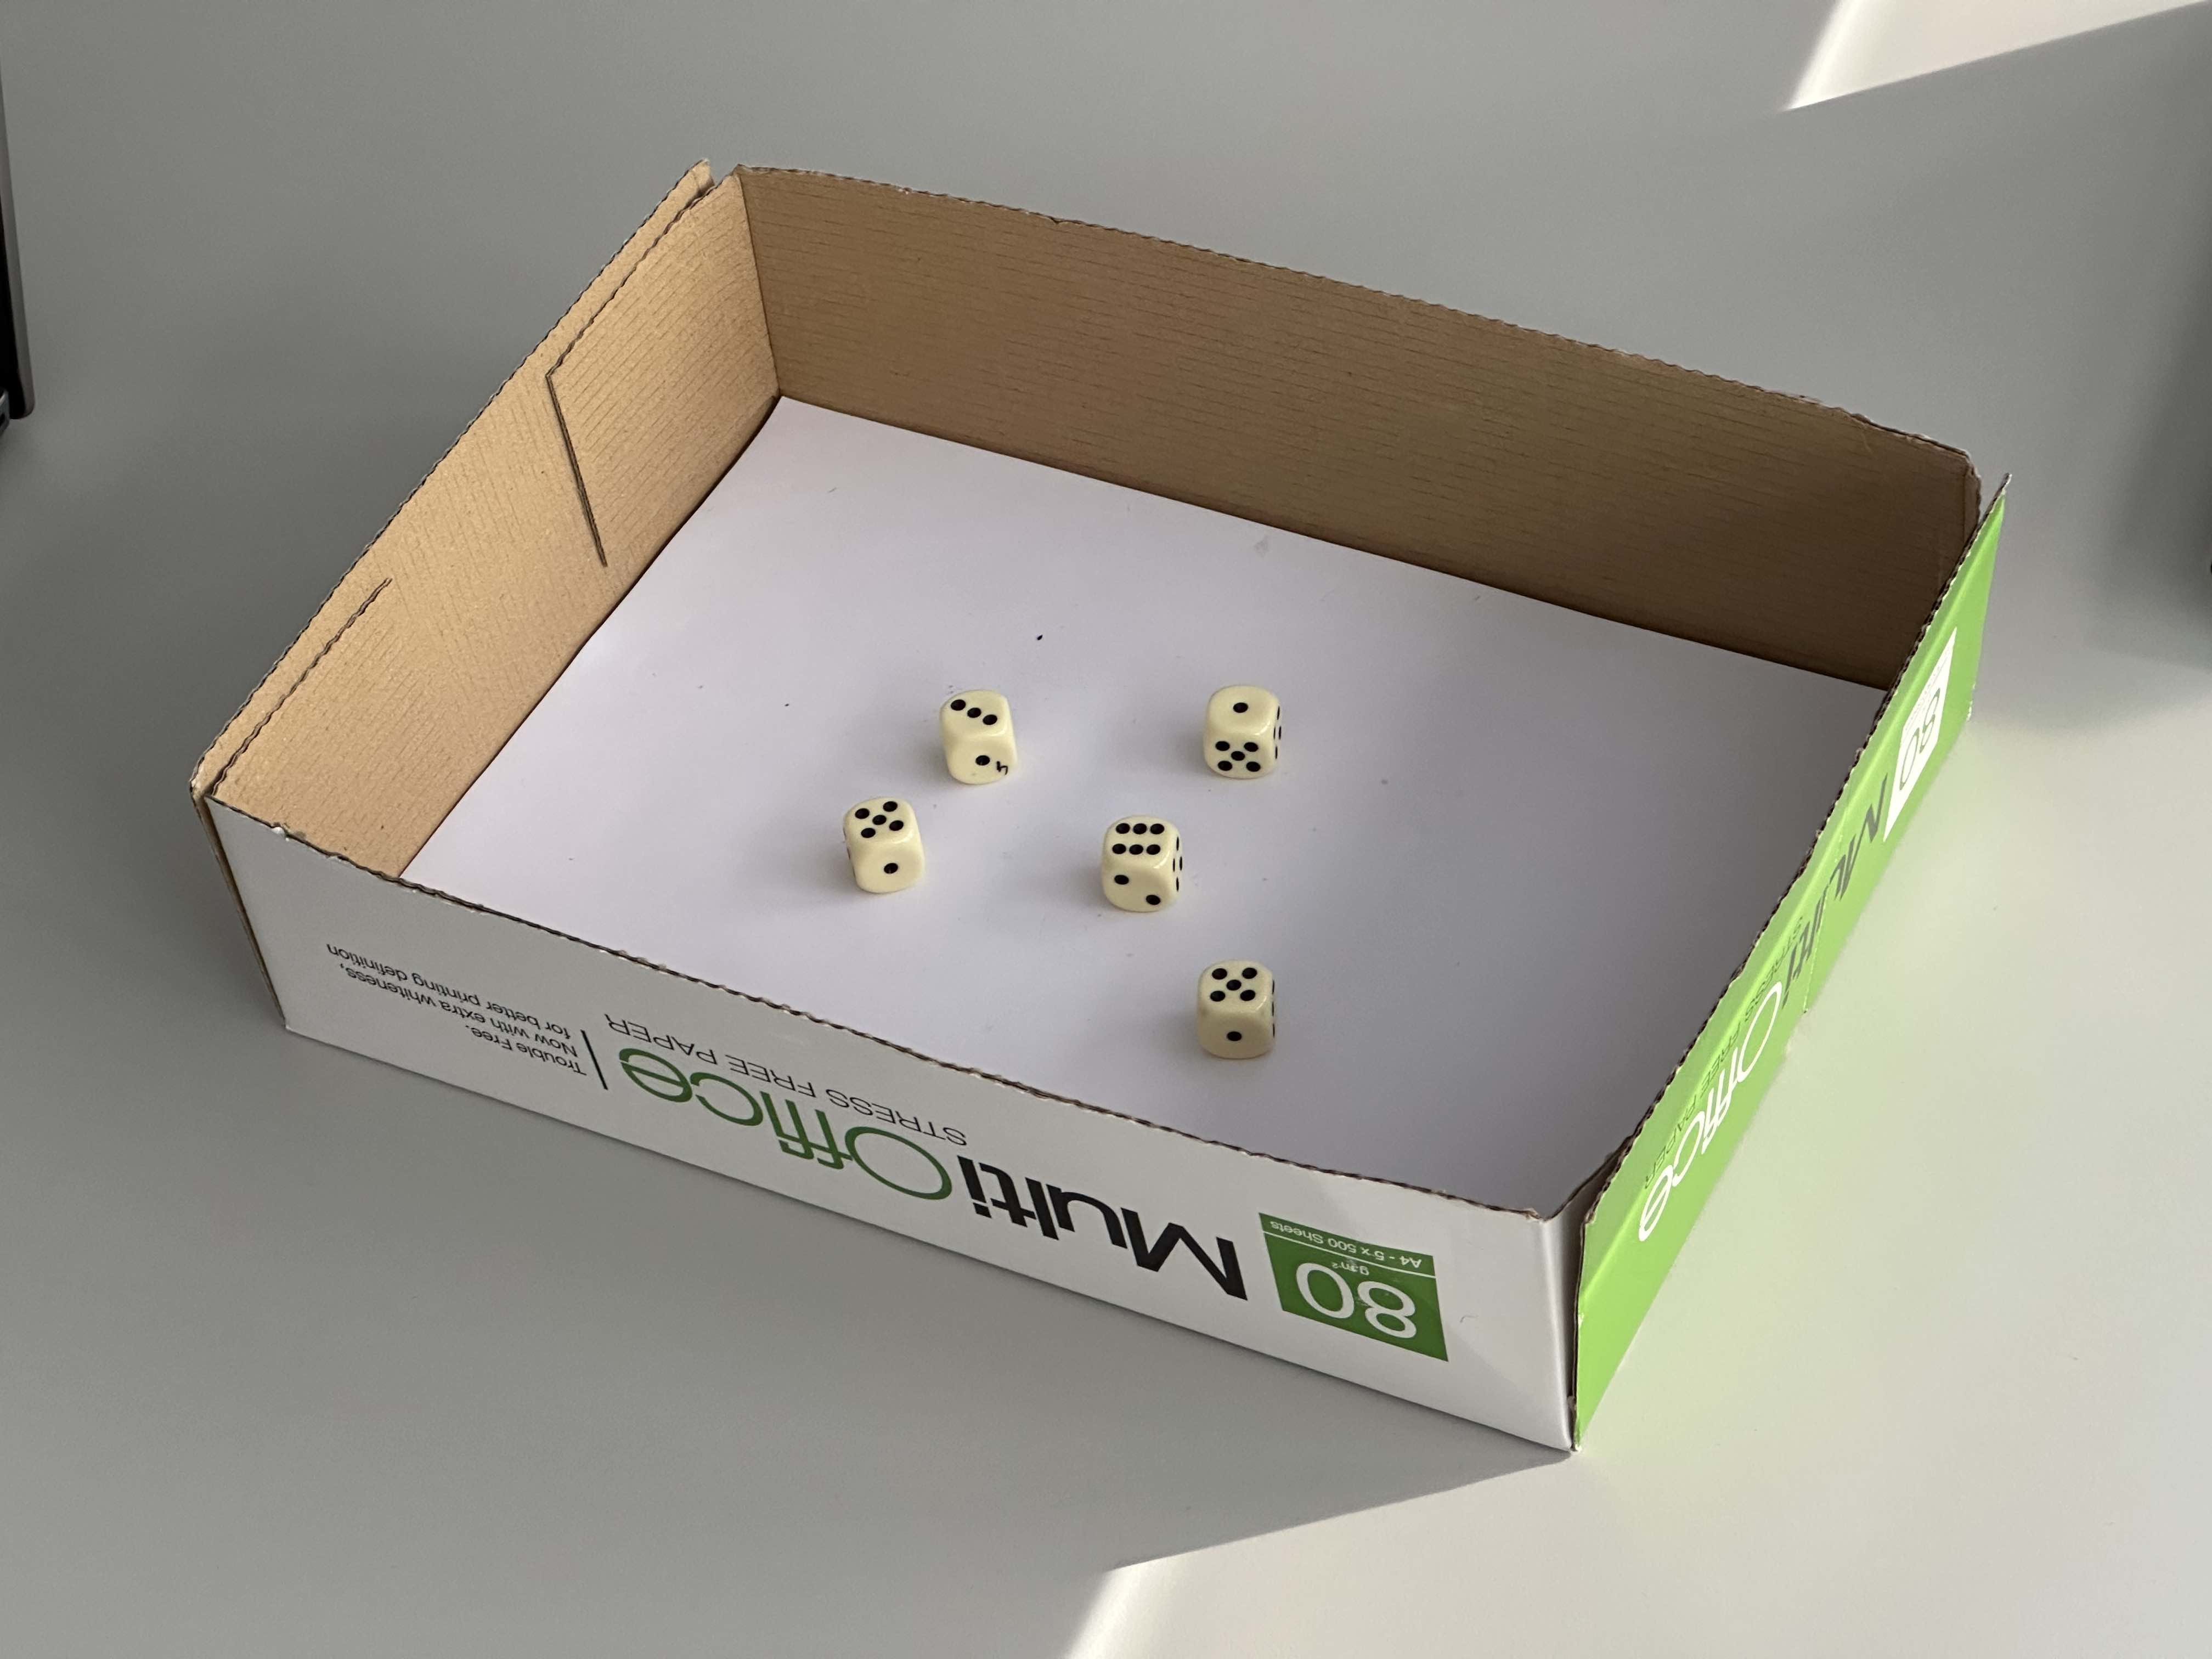
\includegraphics[width=0.5\textwidth]{bilder/IMG_7612.jpg}
    \caption{Würfelteller mit 5 Würfel}
\end{figure}

\subsection{Durchführung}
%//[x] Durchführung
% Wie wurde der Versuch durchgeführt bzw. ausgewertet?
Der Versuch wurde am 18. Oktober 2024 um ca. halb 12 im Raum P122 an der JKU Linz durchgeführt.
Für jeden Messvorgang wurden fünf Würfel gleichzeitig von der Hand in das Würfelteller geworfen. Dabei wurde jeder Würfel 
unabhängig von den anderen betrachtet. Anschließend wurden die Augenzahlen einzeln abgelesen, wobei die Reihenfolge außer 
Acht gelassen wurde. Die abgelesenen Werte wurden im direkten Anschluss an den Würfelvorgang im Laborprotokoll tabellarisch 
dokumentiert. Zur Überprüfung wird handschriftlich ein Histogramm gezeichnet. Es sollen dabei alle Würfel im Würfelteller 
landen und die Würfel geworfen werden, sodass das Würfelergebnis durch den Wurf nicht beeinflussbar ist.

Dieser Vorgang wurde insgesamt 80 mal, für 400 Werte wiederholt. Wobei zur Überprüfung nach 200 Messwerten in OriginPro 
2024 ein vorläufiges Histogramm erstellt wurde. 

\section{Messergebnisse und Auswertung}
%//[x] Messung
% Eigentliche Messung!
% Wie groß sind die Messunsicherheiten („Messfehler“)?
%//[ ] TODO: Anführungszeichen unten?
Die Messwerte sind dem angehängten Laborprotokoll ``Versuch\_Würfeln\_Laborprotokoll.pdf'' zu entnehmen.

%//[x] Auswertung
% evtl. Formeln, etc.
% auf richtges Runden der Werte achten

Zur Auswertung werden zuerst die Werte für den statistischen Mittelwert $m$ und die statistische Standardabweichung 
$s$ berechnet und folglich die aus den Messungen hervorgehenden Stichprobenwerte für den Mittelwert $\mu$ und die 
Standardabweichung $\sigma$.

\begin{equation}
    m = \sum_{i=1}^{6} h_i \cdot x_i
\end{equation}

\begin{equation}
    s = \sqrt{\sum_{i=1}^{6} h_i\cdot(x_i - m)^2}
\end{equation}

\begin{equation}
    \mu = \frac{1}{N}\cdot \sum_{i=1}^{N} x_i
\end{equation}

\begin{equation}
    \sigma = \sqrt{\sum_{i=1}^{N} \frac{(x_i - \mu)^2}{N-1}}
\end{equation}

\begin{equation}
    \sigma_\mu = \sqrt{\frac{1}{N} \sum_{i=1}^{N} \frac{(x_i - \mu)^2}{N - 1}}
\end{equation}

\vspace{0,5cm}

Unter Anwendug von Gl. 1 ergibt sich $m=3,5$ und aus Gl. 2 folgt $s=1,71$.

Weiters wurde OriginPro 2024 verwendet, um den Mittelwert $\mu=3.54$ und die Standardabweichung $\sigma = 1,69$ der Messwerte
nach den Gleichungen 3 und 4 zu ermitteln.
Daraus folgt die Grenzen des $1\sigma$ Vertrauensintervals sind $3,54\pm1,69$.
Die Ermittlung der Unsicherheit des Mittelwertes erfolgte in Excel nach Gleichung 5 und lautet $\sigma_\mu\approx0,09$.

Diese Auswertung wird in Abbildung 2 dargestellt. Darin erkennbar ist ausßerdem eine Normalverteilung, die sich unter Annahme von gleichen $\mu$ und $\sigma$ ergibt.

\begin{figure}[H]
    \centering
    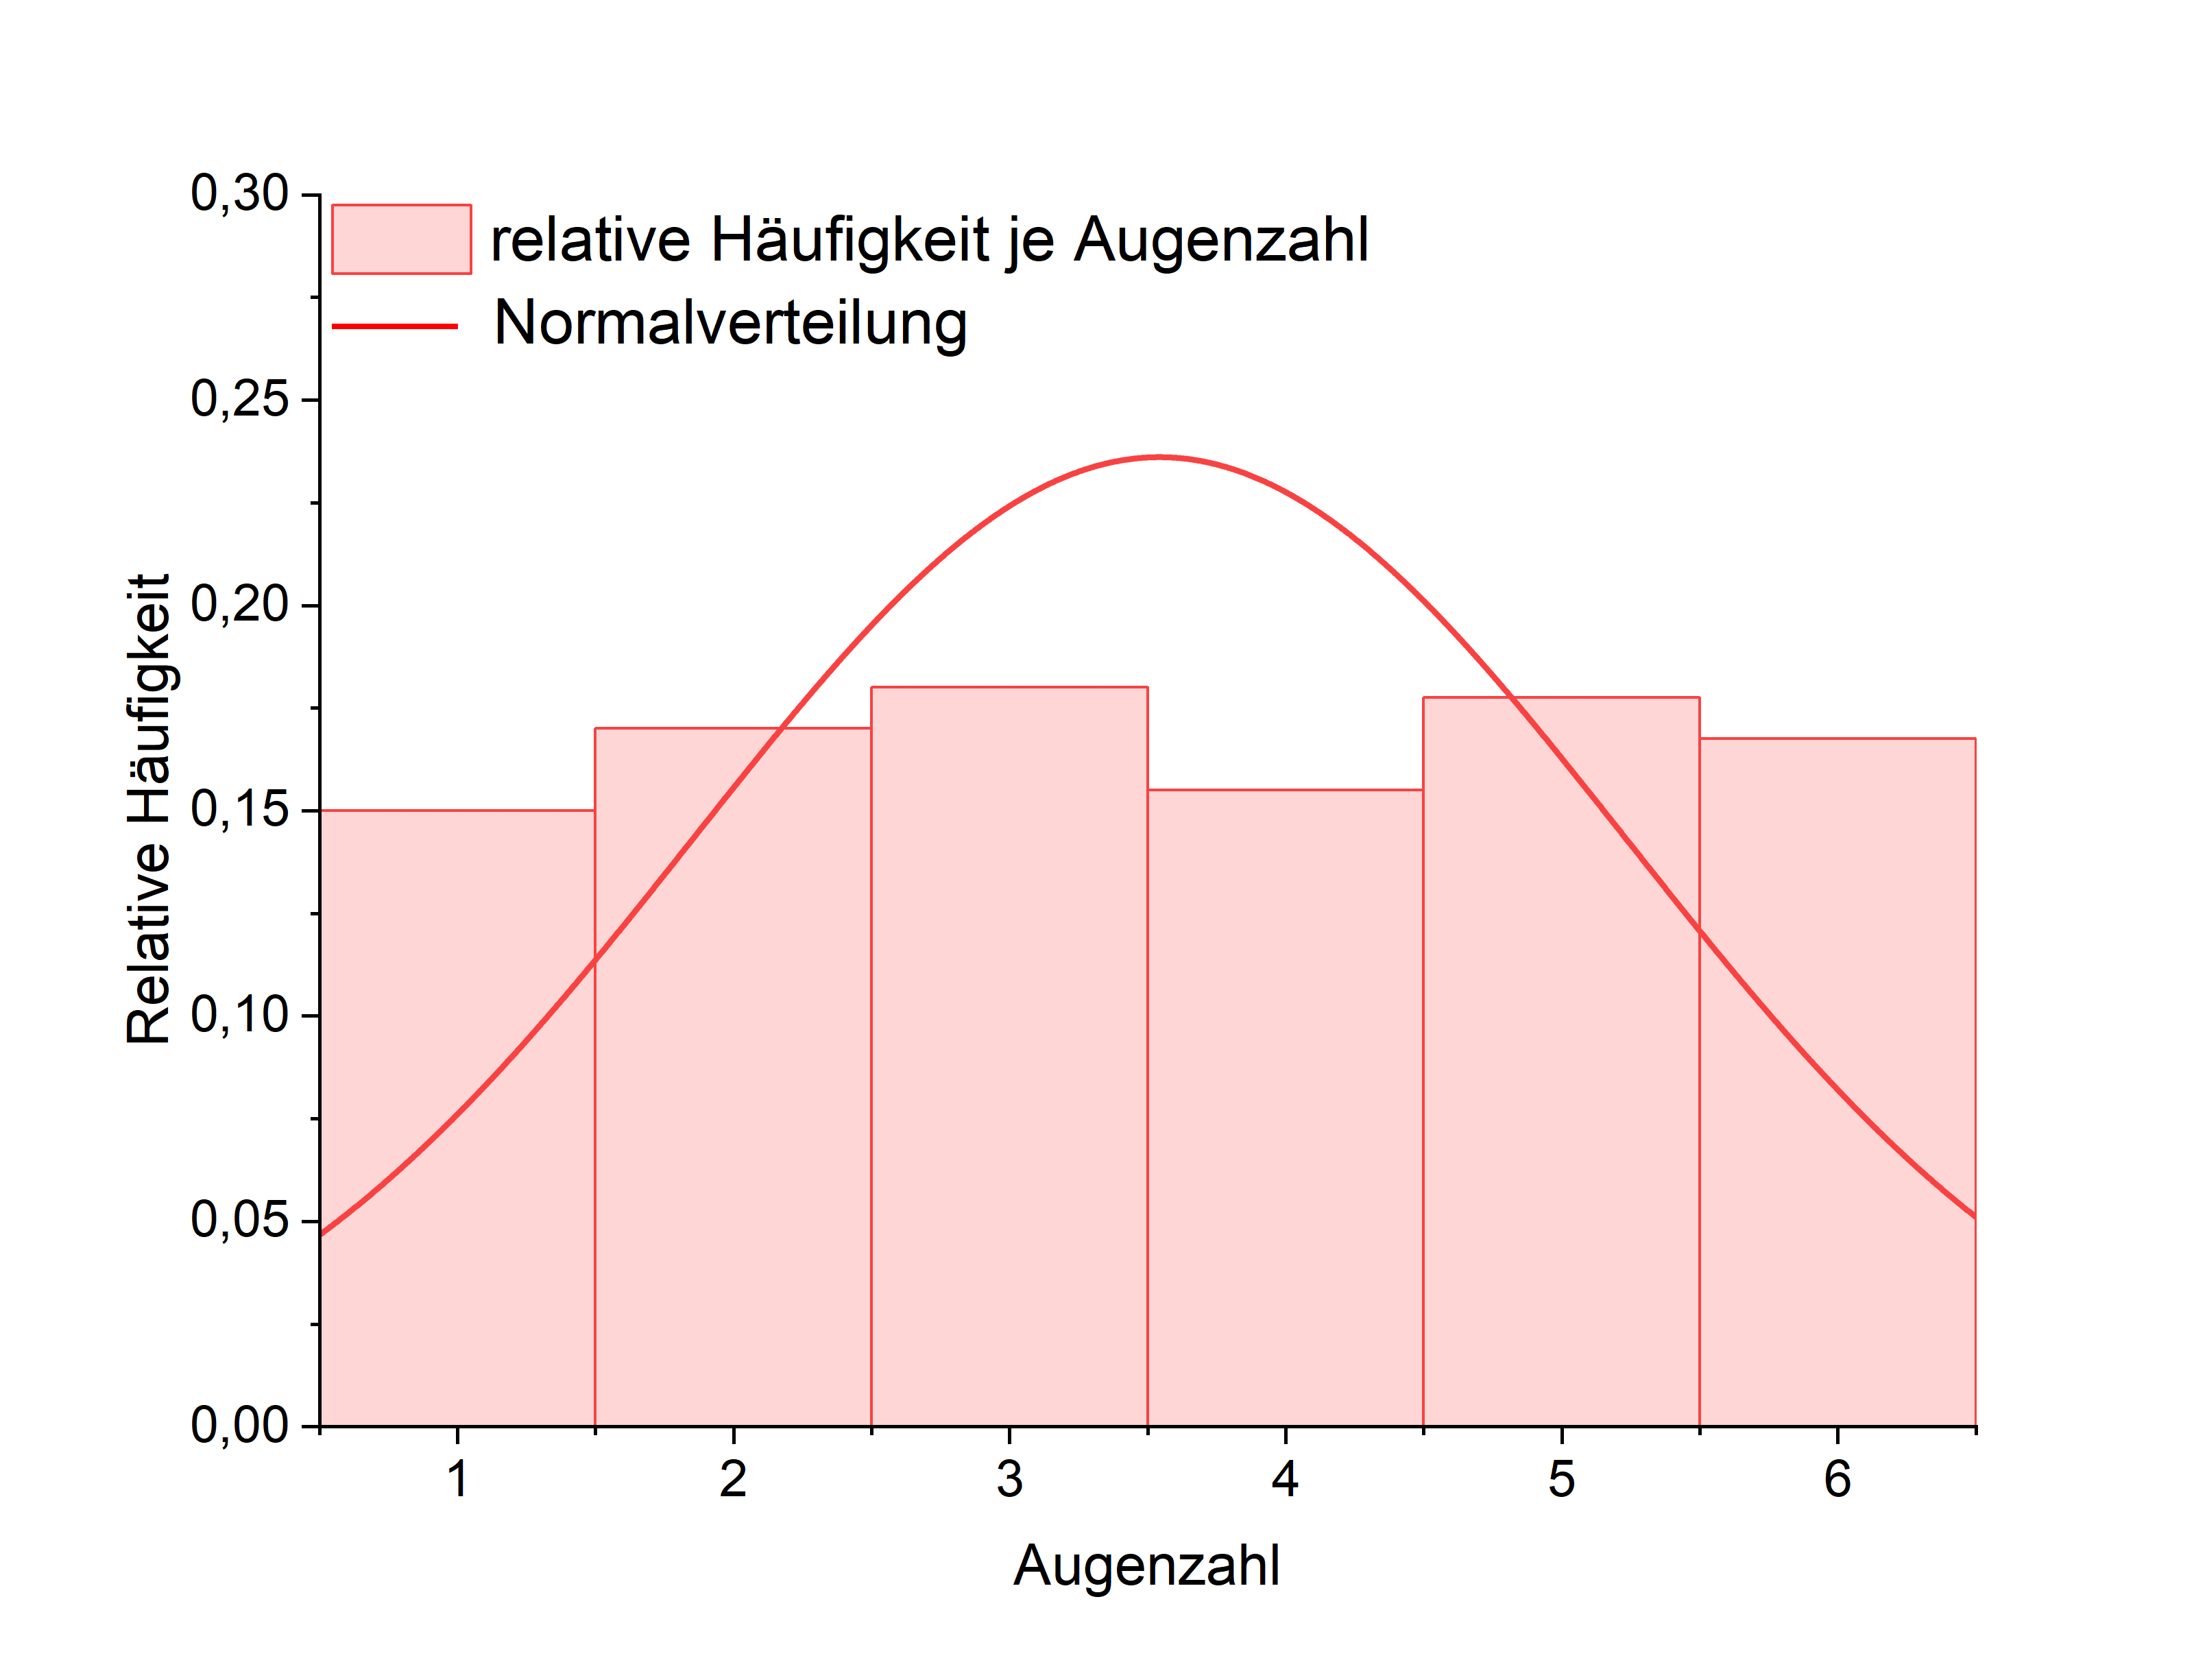
\includegraphics[width=\textwidth]{bilder/Histogramm.png}
    \caption{Histogramm der Messwerte}
\end{figure}

\section{Diskussion}
%//[ ] Diskussion
% Wie vergleicht sich meine Messung mit anderen Messungen/Theorien?
% Ist der Messwert sinnvoll? Stimmt die Größenordnung?
% Wo wurden Fehler gemacht? Was kann man verbessern?
% Gegebenenfalls rekursiv auswerten oder nachmessen!
% ursprüngliche Fragestellung diskutieren
% zB Standardabweichung diskutieren, berechnete Größen nennen

<nach 200 werten Vergelich mit handschriftlichem Histogramm>


\end{document}
